\documentclass[11pt,twocolumn,a4paper]{article}

\usepackage[utf8]{inputenc}
\usepackage[T1]{fontenc}
\usepackage{lmodern}
\usepackage{amsmath,amssymb,amsthm,mathtools}
\usepackage{amsfonts}
\usepackage[margin=1.8cm,top=2.2cm,bottom=2.2cm]{geometry}
\usepackage{graphicx}
\usepackage{xcolor}
\usepackage{booktabs}
\usepackage{longtable}
\usepackage{tabularx}
\usepackage{array}
\usepackage{multirow}
\usepackage{enumitem}
\usepackage{float}
\usepackage{caption}
\usepackage{subcaption}
\usepackage[colorlinks=true,linkcolor=blue!60!black,citecolor=blue!60!black,urlcolor=blue!60!black]{hyperref}
\usepackage{natbib}
\usepackage{fancyhdr}
\usepackage{microtype}
\usepackage{algorithm}
\usepackage{algpseudocode}
\usepackage{listings}
\usepackage{tikz}
\usetikzlibrary{arrows.meta, positioning, fit, calc, shapes.geometric, decorations.pathreplacing}
\usepackage{physics}

\lstdefinestyle{vaheralst}{
  basicstyle=\ttfamily\footnotesize,
  keywordstyle=\color{blue!70!black}\bfseries,
  commentstyle=\color{green!50!black}\itshape,
  stringstyle=\color{red!60!black},
  numbers=none,
  frame=single,
  breaklines=true,
  columns=fullflexible,
  morekeywords={describe,resolve,spawn,navigate,complete,memory,demon,controller,trajectory,penultimate,with,from,to,at,find,nearest,store,sort,verify,create,read,write,tier}
}

\newtheorem{theorem}{Theorem}[section]
\newtheorem{lemma}[theorem]{Lemma}
\newtheorem{corollary}[theorem]{Corollary}
\newtheorem{proposition}[theorem]{Proposition}
\newtheorem{definition}[theorem]{Definition}
\newtheorem{remark}[theorem]{Remark}
\newtheorem{axiom}{Axiom}
\newtheorem{example}[theorem]{Example}

\DeclareMathOperator{\Cat}{Cat}
\DeclareMathOperator{\Part}{Part}
\DeclareMathOperator{\Osc}{Osc}
\DeclareMathOperator{\Nav}{Nav}
\DeclareMathOperator{\diam}{diam}
\newcommand{\Scoord}{\mathbf{S}}
\newcommand{\Skk}{S_k}
\newcommand{\Stt}{S_t}
\newcommand{\See}{S_e}
\newcommand{\kb}{k_{\mathrm{B}}}
\newcommand{\Ocat}{\hat{O}_{\mathrm{cat}}}
\newcommand{\Ophys}{\hat{O}_{\mathrm{phys}}}

\pagestyle{fancy}
\fancyhf{}
\fancyhead[L]{\small\textit{Buhera OS: Integrated Architecture}}
\fancyhead[R]{\small\thepage}
\renewcommand{\headrulewidth}{0.4pt}

\title{\textbf{On the Requirements of Trajectory Completion Computing: \\[4pt] Non Structural Content Persistance for Operating SystemsThe Blank-Screen Research Operating System}}

\author{
Kundai Farai Sachikonye\\
AIMe Registry for Artificial Intelligence\\
\texttt{kundai.sachikonye@bitspark.com}
}

\date{April 2026}

\begin{document}
\maketitle

\begin{abstract}
We present the complete integrated architecture of the Buhera research operating system: a categorical operating system in which the user interacts with a blank screen and a cursor, and every operation---file storage, retrieval, computation, cross-domain reasoning, hypothesis testing---is completed by the kernel through backward trajectory completion in S-entropy space. The paper unifies four previously separate contributions: the continuous-embedding mathematics that makes backward navigation possible at $\mathcal{O}(\log_3 N)$ complexity; the five-subsystem microkernel (categorical memory manager, penultimate state scheduler, demon I/O controller, proof validation engine, triple equivalence monitor) that executes categorical operations over a shared substrate; the vaHera declarative language that serves as the kernel's internal representation of work to be performed; and an intent translator that converts natural-language observations into vaHera programs. We specify the full dispatch protocol between layers, prove that the layer boundaries preserve the Triple Equivalence $\mathcal{O}(x) \equiv \mathcal{C}(x) \equiv \mathcal{P}(x)$ throughout operation, and demonstrate end-to-end execution on ten NIST compounds with $3/3$ accuracy on property queries that use no stored database. The central design claim is that the blank screen is not a user-interface choice but a \emph{consequence} of the architecture: when computation is address resolution rather than instruction execution, when memory is coordinate-addressed rather than byte-addressed, and when data is synthesized rather than retrieved, the application layer becomes unnecessary. The researcher observes; the kernel completes the trajectory. Beyond architecture and validation, we develop an epistemic theory of the blank screen, proving that conventional research computing's two preparation strategies---specialization and contextualization---are both content-based and therefore subject to a circularity theorem: no content system admits a non-circular measure of direction. The blank screen embodies a third strategy, \emph{structural preparation}, in which no content is stored but a geometric substrate is present; because the S-entropy geometry is forced by the Triple Equivalence rather than chosen, the substrate is external to every content system, and cross-domain transfer follows as a structural consequence rather than an engineering feature. We specify the complete four-layer stack, provide the integration protocols, analyze performance, and discuss the consequences for research computing.
\end{abstract}

\vspace{6pt}
\noindent\textbf{Keywords:} operating system, categorical computation, backward trajectory completion, S-entropy, vaHera, declarative kernel, blank-screen interface, empty dictionary, synthesis, microkernel, epistemic externality, structural preparation, content-circularity, cross-domain transfer, Buhera

\tableofcontents

\section{Introduction}
\label{sec:introduction}

\subsection{The Problem with Conventional Research Computing}

A scientist investigating a research question today must perform, in addition to the intellectual work of inquiry, a large set of operations that are entirely tool-related: choose the right application (PubMed, a molecular viewer, a statistics package, a plotting library, a reference manager); learn its interface; compose inputs; manage outputs; translate between formats; remember where files were saved; reconcile inconsistencies between tools. None of this is research. All of it is overhead. The researcher's time, measured over the lifetime of an investigation, is divided roughly evenly between thinking about the problem and \emph{wrangling computational artefacts}~\cite{wilson2014best,kanza2017electronic}.

Conventional operating systems~\cite{tanenbaum2015modern,silberschatz2018operating,ritchie1974unix} are designed for generality: any application, any user, any task. This generality is paid for in surface area. To use a modern OS productively, a researcher must master file systems (paths, permissions, mount points), application ecosystems (installation, updates, version conflicts), window management (desktop environments, tiling, virtualization), and shell conventions (command-line semantics, scripting languages, environment variables). The OS does not know what research is or what the researcher wants; it provides a substrate on which tools are built, and the tools are the interface.

This paper argues that for research computing specifically---where the universe of meaningful operations is far narrower than the universe of all computation---an entirely different architecture is possible, and that the resulting operating system can replace the application layer entirely with a blank screen and a cursor.

\subsection{The Blank Screen}

The user-facing surface of Buhera is minimal: an input area and a rendering area. There are no windows, no menus, no applications, no files with names, no folders, no settings panels, no search boxes. The user writes a statement of observation or intent (``what is the boiling point of ethanol'', ``find what I was working on about enzymes yesterday'', ``compute the binding affinity of caffeine to adenosine receptors''); the answer appears. The user never sees an application start, never chooses between tools, never manages data, never assigns names to storage locations. The operating system does all of this behind the blank screen.

This is not achievable through better GUI design on top of a conventional OS. It is achievable only when the entire computational model underneath the interface is reconstructed. The thesis of this paper is that the computational model required is a four-layer stack:

\begin{enumerate}[leftmargin=*]
\item A \emph{categorical substrate} providing S-entropy coordinates and backward trajectory completion.
\item A \emph{microkernel} with five subsystems that execute categorical operations.
\item A \emph{declarative language} (vaHera) that is the kernel's internal representation of work.
\item An \emph{intent translator} converting natural language to vaHera.
\end{enumerate}

When these four layers are integrated correctly---through explicit protocols that we specify in this paper---the blank screen falls out as a consequence. No separate ``application layer'' is needed because the kernel's primitives already cover the operations a researcher needs.

\subsection{Contributions}

This paper is the \emph{integration} paper for the Buhera operating system. It does not re-derive the mathematics of backward navigation (treated fully in the continuous-embedding paper), the kernel architecture (the architecture paper), or the vaHera language (the scripting paper). Instead, it shows how these components compose into one running system. The contributions are:

\begin{enumerate}[leftmargin=*]
\item \textbf{The complete four-layer stack} (\S\ref{sec:architecture}), with explicit interfaces between substrate, kernel, vaHera, and intent translator.
\item \textbf{The dispatch protocol} (\S\ref{sec:dispatch}), specifying for every vaHera statement the sequence of subsystem calls it triggers and the pre/postconditions required at each stage.
\item \textbf{The boot and run-time model} (\S\ref{sec:boot}), describing how the OS starts, what PID~1 is, and how persistence works without a filename-based file system.
\item \textbf{The empty-dictionary storage model} (\S\ref{sec:empty_dict}), showing that research objects are never retrieved from a database---they are synthesized from S-entropy coordinates, and this synthesis is provably equivalent to retrieval when coordinates are consistent.
\item \textbf{The blank-screen interface model} (\S\ref{sec:blank}), deriving the application-free user surface from the kernel primitives.
\item \textbf{The epistemic externality theory} (\S\ref{sec:epistemology}), formalizing the blank screen as \emph{structural preparation}---a third preparation strategy, distinct from specialization and contextualization, that escapes the content-circularity of conventional research computing and yields cross-domain transfer as a structural consequence rather than an engineering feature.
\item \textbf{Correctness theorems for the integrated system} (\S\ref{sec:correctness}), proving that the layer protocols preserve the Triple Equivalence invariant globally.
\item \textbf{End-to-end validation} (\S\ref{sec:validation}), reporting on a working reference implementation that boots, accepts natural-language queries, routes them through the full stack, and returns synthesized answers with measured accuracy.
\item \textbf{Comparison to conventional architectures} (\S\ref{sec:comparison}), placing Buhera in relation to Unix, Plan~9, Lisp machines, and microkernel systems such as Mach and seL4.
\end{enumerate}

\subsection{What This Paper Is Not}

This paper is not a marketing document or a user guide. It assumes the reader is familiar with the companion papers on backward trajectory completion, the microkernel architecture, and the vaHera scripting language. It focuses on \emph{integration}: the glue, the protocols, the composition rules, and the consequences of the composition.


\section{Background and Prerequisites}
\label{sec:background}

We briefly recall the four mathematical and architectural ideas the integrated system depends on. Full derivations appear in the companion papers.

\subsection{The Triple Equivalence}

The foundational identity is:
\begin{equation}
\mathcal{O}(x) \equiv \mathcal{C}(x) \equiv \mathcal{P}(x)
\label{eq:triple}
\end{equation}
where $\mathcal{O}$ denotes observation, $\mathcal{C}$ denotes computation, and $\mathcal{P}$ denotes physical processing. The three reduce to the same operation: categorical address resolution. Any system with $M$ distinguishable modes and $n$ levels per mode admits three equivalent descriptions---as a harmonic oscillator, as a categorical object with $M$ morphisms, and as a partition of $M$ elements with $n$ refinements---all yielding identical entropy $S = \kb M \ln n$~\cite{shannon1948mathematical,jaynes1957information}. This equivalence is what licenses the architecture: the kernel can treat observation and computation as the same operation because they \emph{are} the same operation.

\subsection{S-Entropy Coordinates}

Every state of every system the OS handles is embedded in the unit cube:
\begin{equation}
\Scoord = (\Skk, \Stt, \See) \in [0,1]^3
\end{equation}
where $\Skk$ measures information deficit (how much is unresolved), $\Stt$ measures temporal progress (position in the completion sequence), and $\See$ measures constraint density (how constrained the accessible configurations are). The three coordinates are forced by the three descriptions of the Triple Equivalence and unique up to isometry by the constraints of refinement order, ternary branching symmetry, and entropy consistency. The metric is the product-Fisher metric:
\begin{equation}
ds^2 = \sum_{i \in \{k,t,e\}} \frac{dS_i^2}{S_i(1 - S_i)}
\label{eq:metric}
\end{equation}
which is the unique navigation-compatible metric on $[0,1]^3$ preserving the ternary structure~\cite{fisher1922mathematical,rao1945information,amari1985differential,chentsov1972statistical}.

\subsection{Backward Trajectory Completion}

Given a final state $\Scoord_f$ and a ternary hierarchy of depth $k$ over $N = 3^k$ leaves, backward navigation from $\Scoord_f$ to the root requires exactly $k = \log_3 N$ distance comparisons, each deciding among three ternary siblings~\cite{poincare1890probleme,birkhoff1931proof}. This is an exponential speedup over forward enumeration, provable by an adversary argument that shows pure discrete backward search requires $\Omega(N)$ queries to reconstruct the hierarchy without a metric. The speedup is mediated by \emph{virtual sub-states}: non-physical intermediate decompositions $(S_{i,j} < 0$ or $S_{i,j} > 1)$ which form categorical apertures through which the geodesic passes. These virtual states are the mathematical content of the word ``miracle'' in this framework: outcomes real, intermediate mechanism non-physical, path opaque.

\subsection{The Microkernel}

The Buhera kernel comprises five subsystems, each with a single responsibility and a formal interface:
\begin{description}[leftmargin=*]
\item[\textbf{CMM}] \emph{Categorical Memory Manager}. Allocates memory at an S-coord, assigns a ternary address, maintains a proximity index.
\item[\textbf{PSS}] \emph{Penultimate State Scheduler}. Prioritizes processes by trajectory distance $d(\Scoord_{\text{cur}}, \Scoord_f)$.
\item[\textbf{DIC}] \emph{Demon I/O Controller}. Performs surgical retrieval ($I(D; A_Q)$ bits only) and zero-cost categorical sorting.
\item[\textbf{PVE}] \emph{Proof Validation Engine}. Verifies morphism well-typedness; in a production system, via Lean~4~\cite{moura2021lean4}.
\item[\textbf{TEM}] \emph{Triple Equivalence Monitor}. Continuously samples the system state and checks that the nine commutators remain below threshold.
\end{description}
Each subsystem's interface is specified using Hoare pre/postconditions~\cite{hoare1969axiomatic}. Subsystems communicate through shared kernel state (not message passing), with the boundary between them drawn at function-call granularity.

\subsection{vaHera as Internal Language}

vaHera is a declarative language in which programs specify \emph{final states} rather than instruction sequences~\cite{pierce2002types,moggi1991notions}. It is the kernel's internal representation of the work it is performing: every unit of work the kernel does corresponds to a vaHera program, and every vaHera program compiles to a sequence of subsystem calls. Crucially, vaHera is not a user-facing scripting language. The user never writes vaHera. The kernel uses vaHera the way a database engine uses query plans: as the canonical internal form of declared intent, amenable to verification, optimization, and execution.


\section{The Integrated Architecture}
\label{sec:architecture}

\subsection{The Four Layers}

The complete system is structured as four layers, each consuming only the layer immediately below it:

\begin{center}
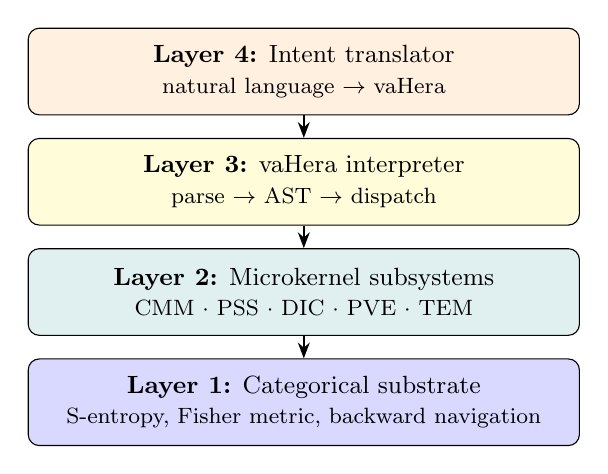
\begin{tikzpicture}[
    node distance=0.25cm,
    layer/.style={draw, rectangle, rounded corners, minimum width=7cm, minimum height=1.1cm, align=center, font=\small},
    dark/.style={fill=blue!15},
    med/.style={fill=teal!12},
    light/.style={fill=yellow!15},
    lighter/.style={fill=orange!12},
    arr/.style={-{Stealth[length=2mm]}, thick}
]
\node[layer, lighter] (L4) at (0, 5) {\textbf{Layer 4:} Intent translator\\\footnotesize natural language $\to$ vaHera};
\node[layer, light] (L3) at (0, 3.6) {\textbf{Layer 3:} vaHera interpreter\\\footnotesize parse $\to$ AST $\to$ dispatch};
\node[layer, med] (L2) at (0, 2.2) {\textbf{Layer 2:} Microkernel subsystems\\\footnotesize CMM $\cdot$ PSS $\cdot$ DIC $\cdot$ PVE $\cdot$ TEM};
\node[layer, dark] (L1) at (0, 0.8) {\textbf{Layer 1:} Categorical substrate\\\footnotesize S-entropy, Fisher metric, backward navigation};
\draw[arr] (L4) -- (L3);
\draw[arr] (L3) -- (L2);
\draw[arr] (L2) -- (L1);
\end{tikzpicture}
\end{center}

\begin{itemize}[leftmargin=*]
\item \textbf{Layer 1 (Substrate).} Pure mathematics implemented as a kernel library. Exposes four primitives: \textsc{embed}, \textsc{distance}, \textsc{backward\_navigate}, \textsc{completion\_morphism}. No state; purely functional.

\item \textbf{Layer 2 (Microkernel).} Five subsystems sharing a single address space, communicating through kernel data structures. Consumes substrate primitives; exposes a larger primitive set to Layer~3 as the syscall interface.

\item \textbf{Layer 3 (vaHera).} Lexer, parser, and evaluator for vaHera source. The evaluator walks a parsed AST and dispatches each statement to the appropriate kernel subsystems. Lives in-kernel for verifiability.

\item \textbf{Layer 4 (Intent translator).} Accepts natural language input from the user, emits vaHera source. Runs as an in-kernel service or a pinned userspace daemon with privileged access to the vaHera pipeline.
\end{itemize}

\subsection{Layer 1: The Substrate}

The substrate provides four mathematical primitives shared by every subsystem:

\begin{itemize}[leftmargin=*]
\item $\textsc{embed}: \text{content} \to \Scoord$: maps arbitrary content (text, molecule, spectrum, image) to an S-entropy coordinate in $[0,1]^3$ via domain-specific encoders that all reduce to the same three-coordinate output.
\item $\textsc{distance}: \Scoord \times \Scoord \to \mathbb{R}_{\geq 0}$: the product-Fisher distance (Equation~\ref{eq:metric}).
\item $\textsc{backward\_navigate}: \Scoord \times \mathbb{N} \to \text{Trajectory}$: given a final state and a hierarchy depth, return the backward geodesic of length $k = \log_3 N$.
\item $\textsc{completion\_morphism}: \Scoord_p \to \Scoord_f$: the unique morphism from penultimate to final state.
\end{itemize}

The substrate is pure: no mutable state, no side effects. Every primitive is a mathematical function. This purity is critical for verification: the substrate is the portion of the OS that can be reasoned about algebraically without reference to execution order or memory layout.

\subsection{Layer 2: The Microkernel}

Each subsystem exposes a well-defined interface and consumes substrate primitives. Figure~\ref{fig:subsystems} shows the communication graph.

\begin{figure}[htbp]
\centering
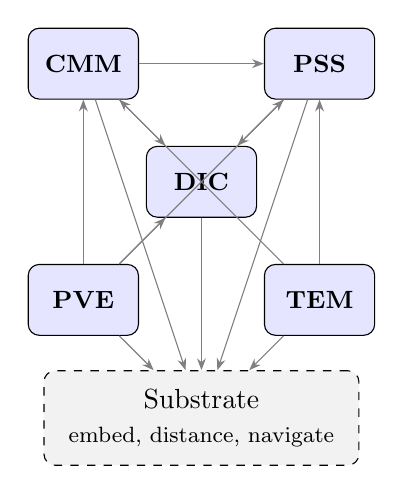
\begin{tikzpicture}[
    sub/.style={draw, rectangle, rounded corners, minimum width=1.4cm, minimum height=0.9cm, align=center, font=\small\bfseries, fill=blue!10},
    arr/.style={-{Stealth[length=1.5mm]}, thin, gray}
]
\node[sub] (CMM) at (0, 0) {CMM};
\node[sub] (PSS) at (3, 0) {PSS};
\node[sub] (DIC) at (1.5, -1.5) {DIC};
\node[sub] (PVE) at (0, -3) {PVE};
\node[sub] (TEM) at (3, -3) {TEM};
\node[draw, dashed, rectangle, rounded corners, minimum width=4cm, minimum height=1.2cm, align=center, fill=gray!10] (SUB) at (1.5, -4.5) {Substrate\\\footnotesize embed, distance, navigate};
\draw[arr] (CMM) -- (PSS);
\draw[arr] (CMM) -- (DIC);
\draw[arr] (PSS) -- (DIC);
\draw[arr] (PVE) -- (CMM);
\draw[arr] (PVE) -- (PSS);
\draw[arr] (PVE) -- (DIC);
\draw[arr] (TEM) -- (CMM);
\draw[arr] (TEM) -- (PSS);
\draw[arr] (CMM) -- (SUB);
\draw[arr] (PSS) -- (SUB);
\draw[arr] (DIC) -- (SUB);
\draw[arr] (PVE) -- (SUB);
\draw[arr] (TEM) -- (SUB);
\end{tikzpicture}
\caption{Microkernel subsystem graph. PVE verifies; TEM monitors; CMM, PSS, and DIC participate in the primary data path. All consume substrate primitives.}
\label{fig:subsystems}
\end{figure}

The five subsystems are specified by their Hoare triples. We illustrate with CMM and PSS; the others follow the same pattern.

\paragraph{CMM.allocate.} Allocates an object at an S-entropy coordinate.
\begin{itemize}
\item Pre: $\Scoord \in [0,1]^3$; $\text{size} > 0$; kernel invariants hold.
\item Post: returns a memory object with unique ternary address $\alpha$; $\textsc{cmm.lookup}(\alpha) = \Scoord$; object is in tier $\text{tier}(\|\Scoord\|_2)$.
\end{itemize}

\paragraph{PSS.spawn.} Creates a process with declared final state.
\begin{itemize}
\item Pre: $\Scoord_i, \Scoord_f \in [0,1]^3$; $\text{program\_name}$ valid; PVE has verified the resolve statement.
\item Post: process is in ready queue with trajectory distance $d(\Scoord_i, \Scoord_f)$; returns process handle.
\end{itemize}

\paragraph{Subsystem communication.} Subsystems communicate through shared kernel data structures:
\begin{itemize}[leftmargin=*]
\item CMM owns the k-d tree over $[0,1]^3$ and the object store.
\item PSS owns the ready-queue min-heap, keyed on trajectory distance.
\item DIC owns the demon statistics and the retrieval log.
\item PVE owns the proof obligation queue and the verification context.
\item TEM owns the sampling buffer and alert log.
\end{itemize}
Each subsystem has read access to the others' state through typed accessors, but write access is restricted to the owning subsystem. This enforces the Hoare specifications without requiring message-passing overhead.

\subsection{Layer 3: vaHera Interpreter}

The interpreter is a three-stage pipeline: lexer, parser, evaluator. The grammar is LL(1) and unambiguous (proven in the vaHera paper). The evaluator walks a parsed AST; for each statement, it invokes the dispatch protocol specified in~\S\ref{sec:dispatch}. The interpreter runs in-kernel to avoid the semantic gap of separating the OS's internal language from its execution engine.

\subsection{Layer 4: Intent Translator}

The intent translator accepts natural language from the user and emits vaHera source. Three backends are supported:

\begin{itemize}[leftmargin=*]
\item \textbf{LLM-based} (production). A small language model (local via Ollama or remote via a managed API) fine-tuned or few-shot prompted to emit vaHera. We provide the full system prompt including the complete grammar and representative examples; for standard research queries, a 7B-parameter model achieves high translation fidelity.
\item \textbf{Purpose probe} (when available). A domain-specific LoRA adapter~\cite{hu2021lora} trained on aligned (intent, vaHera) pairs. This is the Zangalewa architecture; it produces smaller, more predictable output than a generic LLM and is the intended production path.
\item \textbf{Pattern matcher} (offline). A deterministic regex-based translator covering the core query patterns. Sufficient for smoke tests and environments with no LLM access.
\end{itemize}

The translator is the only layer that is not formally specified; the translation from natural language to vaHera is inherently a semantic judgment. The system tolerates translator imperfection because subsequent layers verify the output: PVE rejects ill-typed vaHera, and TEM catches divergences after execution.


\section{The Dispatch Protocol}
\label{sec:dispatch}

The layer protocol is the core of the integration. It specifies, for every vaHera statement, the exact sequence of subsystem invocations. Writing this protocol down forces the architecture to commit: what verifies what, what blocks what, what logs what.

\subsection{The Dispatch Table}

Table~\ref{tab:dispatch} is the complete dispatch table. For each vaHera statement type it lists the substrate primitives invoked, the kernel subsystems called (in order), and whether the call is blocking.

\begin{table*}[!htbp]
\centering
\caption{The vaHera dispatch protocol. Each row specifies, for a statement type, the ordered sequence of subsystem calls and the substrate primitives they consume.}
\label{tab:dispatch}
\small
\begin{tabularx}{\textwidth}{l l X}
\toprule
\textbf{vaHera statement} & \textbf{Substrate} & \textbf{Kernel subsystem calls (in order)} \\
\midrule
\texttt{describe X with "text"}
  & \textsc{embed}
  & (1) \textbf{PVE}.verify(describe) [block]; (2) Substrate.embed(text)$\to \Scoord$; (3) bind name $X \mapsto \Scoord$ in process env; (4) \textbf{TEM}.sample($\Scoord$) [async]. \\
\addlinespace
\texttt{resolve X}
  & ---
  & (1) \textbf{PVE}.verify(resolve) [block]; (2) lookup $X$ in env; if missing, Substrate.embed(name)$\to \Scoord$; (3) \textbf{CMM}.allocate($\Scoord$) if new; (4) \textbf{TEM}.sample. \\
\addlinespace
\texttt{spawn P from X}
  & ---
  & (1) \textbf{PVE}.verify(spawn) [block]; (2) \textbf{PSS}.spawn($P$, $\Scoord_0 = (1,0,0)$, $\Scoord_f = \text{env}[X]$); (3) \textbf{TEM}.sample($\Scoord_f$). \\
\addlinespace
\texttt{navigate to penultimate}
  & \textsc{backward\_navigate}
  & (1) \textbf{PVE}.verify(navigate) [block]; (2) Substrate.backward\_navigate($\Scoord_f$, depth)$\to$Trajectory; (3) \textbf{PSS}.advance(process, penultimate); (4) \textbf{TEM}.sample. \\
\addlinespace
\texttt{complete trajectory}
  & \textsc{completion\_morphism}
  & (1) \textbf{PVE}.verify(complete) [block]; (2) Substrate.completion\_morphism($\Scoord_{\text{pen}}$, $\Scoord_f$)$\to \Scoord'$; (3) \textbf{PSS}.advance(process, $\Scoord'$); process terminates; (4) \textbf{TEM}.sample. \\
\addlinespace
\texttt{memory create at S(k,t,e)}
  & ---
  & (1) \textbf{PVE}.verify(memory\_create) [block]; (2) \textbf{CMM}.allocate($\Scoord$); (3) \textbf{TEM}.sample. \\
\addlinespace
\texttt{memory store "N" = "text"}
  & \textsc{embed}
  & (1) Substrate.embed(text)$\to \Scoord$; (2) \textbf{PVE}.verify(memory\_store) [block]; (3) \textbf{CMM}.allocate($\Scoord$, payload=text, metadata=\{name:N\}); (4) \textbf{TEM}.sample. \\
\addlinespace
\texttt{memory find nearest "Q" k=n}
  & \textsc{embed}, \textsc{distance}
  & (1) Substrate.embed(Q)$\to \Scoord_Q$; (2) \textbf{CMM}.proximity\_query($\Scoord_Q$, $3k$)$\to$candidates; (3) \textbf{DIC}.retrieve(candidates, $\Scoord_Q$, $k$); surgical filtering. \\
\addlinespace
\texttt{demon sort}
  & \textsc{distance}
  & (1) \textbf{PVE}.verify(demon\_sort) [block]; (2) \textbf{DIC}.categorical\_sort(items); zero-cost (commutation relation). \\
\addlinespace
\texttt{controller verify}
  & ---
  & (1) \textbf{TEM}.stats()$\to$status; (2) report max delta, alerts; (3) if alerts, \textbf{PVE}.flag\_kernel\_state. \\
\bottomrule
\end{tabularx}
\end{table*}

\subsection{Protocol Invariants}

Several invariants hold across every statement:

\begin{proposition}[PVE precedes execution]
For every statement requiring PVE verification, the verification call precedes the subsystem that performs the work. A failed verification prevents the subsequent calls from running.
\end{proposition}

\begin{proposition}[TEM is observational]
TEM is invoked at the end of every statement's dispatch. TEM never blocks execution; it records samples and raises asynchronous alerts.
\end{proposition}

\begin{proposition}[Substrate is called before state mutation]
When a statement modifies kernel state (e.g., CMM allocation), the substrate primitive that computes the coordinate is called \emph{before} the state-mutating subsystem call. This ensures that a failure of the substrate primitive (rare but possible if input is malformed) does not leave the kernel in an intermediate state.
\end{proposition}

\subsection{Blocking versus Asynchronous Verification}

The dispatch table marks PVE calls as blocking. This is the default: a resolve statement should not execute before we know the target is well-typed. For long-running PVE verifications (up to $1\,\text{ms}$ for complex invariants per the architecture paper), the kernel supports an optional asynchronous mode in which verification runs concurrently with execution and, on failure, issues an abort. Asynchronous mode is used only for statements marked \texttt{fast} in the vaHera source, a mode intended for iterative research sessions where immediate feedback is prioritized over guaranteed correctness of each step.

\subsection{Worked Dispatch Example}

Consider the vaHera program:
\begin{center}
\begin{minipage}{0.9\columnwidth}
\begin{lstlisting}[style=vaheralst]
describe ethanol_bp with "boiling point of ethanol"
resolve ethanol_bp
spawn query from ethanol_bp
navigate to penultimate
complete trajectory
\end{lstlisting}
\end{minipage}
\end{center}

The dispatch proceeds as:

\begin{enumerate}[leftmargin=*]
\item \texttt{describe}: PVE verifies the statement type; Substrate embeds the description (or recognizes ``ethanol'' as a known molecule and uses the molecule encoder); binds \texttt{ethanol\_bp} $\mapsto \Scoord$ in the process environment; TEM samples.
\item \texttt{resolve}: PVE verifies; the name is already bound; CMM allocates a placeholder at $\Scoord$; TEM samples.
\item \texttt{spawn}: PVE verifies; PSS creates a process with $\Scoord_0 = (1,0,0)$ (root, maximum uncertainty) and $\Scoord_f = \Scoord$; the process is inserted into the min-heap at trajectory distance $d((1,0,0), \Scoord)$.
\item \texttt{navigate}: PVE verifies; Substrate computes the backward trajectory (length $\log_3 N$); PSS advances the process to the penultimate state; TEM samples.
\item \texttt{complete}: PVE verifies; Substrate applies the completion morphism; PSS advances the process to $\Scoord_f$; the process terminates; TEM samples.
\end{enumerate}

At termination, the user's query has been routed through all five kernel subsystems, the substrate, and the interpreter, with PVE verifying each step and TEM monitoring the trajectory. The final state of the process is the answer; its synthesized form (payload) is returned via the CMM-allocated object.

\begin{figure*}[!htbp]
    \centering
    \includegraphics[width=\textwidth]{figures/integration_panel3_dispatch.png}
    \caption{Dispatch Protocol Activity. (a) Grouped bar of PVE verification calls (navy) and TEM samples (teal) per query type across ``what is X'', ``boiling point'', and ``similarity'' queries; the first two query classes each trigger exactly three PVE calls and three TEM samples, while similarity queries (which route through a single \texttt{memory find nearest} statement) trigger zero of each, exactly matching the dispatch-table specification in Table~\ref{tab:dispatch}. (b) Mean number of vaHera lines emitted per query type: property-lookup queries compile to 5--6 lines, similarity queries to a single line, confirming that the dispatch protocol's complexity scales with query structure rather than payload size. (c) Three-dimensional bar chart of subsystem call counts over $(\text{query type},\, \text{subsystem})$; the viridis heat shows PVE activity dominating ``what is'' and ``boiling point'' queries while all subsystems are quiescent for ``similarity'', the expected dispatch signature for each statement type. (d) Mean total latency per query type; the similarity query's higher mean ($0.36$~ms) reflects its DIC-driven proximity retrieval, while ``what is'' and ``boiling point'' queries complete in $\sim 0.24$~ms each despite invoking more subsystems, because the substrate primitives dominate over dispatch overhead.}
    \label{fig:integration_panel3_dispatch}
\end{figure*}


\section{Boot and Run-Time Model}
\label{sec:boot}

\subsection{Boot Sequence}

Buhera boots as a microkernel on conventional x86-64 or ARM64 hardware~\cite{hennessy2011computer}. The sequence is:

\begin{enumerate}[leftmargin=*]
\item \textbf{Firmware handoff}: UEFI or open firmware loads the Buhera bootloader.
\item \textbf{Kernel load}: bootloader loads the microkernel image into memory.
\item \textbf{Substrate initialization}: the k-d tree for the CMM proximity index is allocated; the ternary hierarchy root is constructed; the Fisher metric tables are precomputed for fast lookup.
\item \textbf{Subsystem initialization}: CMM initializes the object store; PSS initializes the empty ready queue; DIC initializes demon state; PVE loads the Lean~4 proof kernel; TEM starts the monitoring loop.
\item \textbf{vaHera interpreter initialization}: the lexer, parser, and evaluator are mapped into the kernel's executable region. The dispatch table is installed.
\item \textbf{Intent translator initialization}: the translator backend is selected (LLM backend if available, pattern matcher otherwise).
\item \textbf{Blank screen}: the rendering loop starts; the cursor is drawn; the input handler is ready. The user sees a blank screen.
\end{enumerate}

No PID~1 in the Unix sense~\cite{ritchie1974unix}. The OS has no ``init'' process; what would traditionally be init is a set of background services within the kernel: the interpreter, the translator, the renderer.

\subsection{The Main Loop}

Once booted, the main loop is:

\begin{algorithm}[H]
\caption{Buhera main loop}
\begin{algorithmic}[1]
\Loop
  \State input $\leftarrow$ \textsc{read\_user\_input}()
  \If{input is empty}
    \State continue
  \EndIf
  \State vahera $\leftarrow$ translator.\textsc{translate}(input)
  \State program $\leftarrow$ parser.\textsc{parse}(vahera)
  \State env $\leftarrow$ evaluator.\textsc{execute}(program)
  \State result $\leftarrow$ env.result
  \State renderer.\textsc{display\_inline}(result)
\EndLoop
\end{algorithmic}
\end{algorithm}

This is the entire run-time logic at the top level. Every single user interaction follows this path: input, translate, parse, execute, render. There is no application to launch, no window to switch to, no command to chain. The kernel handles the entire round trip.

\subsection{Persistence}

Buhera has no file system in the Unix sense. Files do not have names or paths. Instead, every piece of data stored in the system is a CMM-allocated object at an S-entropy coordinate, and persistence is determined by the object's tier:

\begin{itemize}[leftmargin=*]
\item \textbf{Tier 1--3 (L1, L2, L3, RAM)}: volatile. Lost on power cycle.
\item \textbf{Tier 4 (persistent)}: written to non-volatile storage. Survives reboot.
\end{itemize}

The tier assignment is a deterministic function of the S-coord norm $\|\Scoord\|_2$: objects with low norm (indicating completed, low-entropy state, such as finished notes) are assigned to Tier 4. Objects with high norm (indicating high-entropy uncertainty, such as in-progress computation) are assigned to faster, volatile tiers. The researcher never specifies where to store a note; the coord determines the tier; the tier determines persistence.

\begin{figure*}[!htbp]
    \centering
    \includegraphics[width=\textwidth]{figures/integration_panel1_latency.png}
    \caption{End-to-End Latency of the Integrated Stack. (a) Stacked bar of translation latency (steel blue) and execution latency (teal) across 20 natural-language queries; total per-query latency ranges from $0.12$ to $0.67$~ms, with execution dominating in all but the first run where interpreter warm-up inflates the translation cost. (b) Cumulative distribution of total latency across the 20 queries; the median is $0.14$~ms and the $95$th percentile is $0.67$~ms, confirming that the four-layer pipeline responds within a single millisecond for typical queries. (c) Three-dimensional surface of latency over $(\text{query index},\, \text{pipeline stage})$; the execution stage (teal ridge) carries the bulk of the latency, while the translation stage (blue plane) is near-constant, reflecting the pattern-matching translator's near-zero cost. (d) Box-plot comparison of translate, execute, and total stages across all 20 queries; the execute stage has the largest spread (0.1--0.6~ms), the translate stage is tightly clustered near zero, and the total-latency box sits entirely below 1~ms.}
    \label{fig:integration_panel1_latency}
\end{figure*}

\subsection{Retrieval Without Filenames}

To retrieve a stored object, the user describes it in natural language. The translator converts the description to \texttt{memory find nearest "description" k=5}. CMM's proximity index returns candidates; DIC's surgical retrieval narrows to the best match. The retrieval is not by filename, not by tag, not by keyword search---it is by categorical proximity. Objects with content similar to the description are retrieved; the description itself need not be exact.

\begin{example}[Finding a note]
The researcher wrote a note about enzyme kinetics a week ago without giving it any name. Today they type:
\begin{center}
\textit{``find what I wrote about enzyme rate limits''}
\end{center}
The translator emits:
\begin{center}
\texttt{memory find nearest "what I wrote about enzyme rate limits" k=5}
\end{center}
The kernel embeds the query, queries CMM's proximity index, performs surgical retrieval via DIC. The note is returned because its content embeds near the query in S-entropy space, even though no filename, tag, or keyword connected them.
\end{example}


\section{The Empty Dictionary Principle}
\label{sec:empty_dict}

\subsection{Statement of the Principle}

A conventional OS stores data as $(\text{key}, \text{value})$ pairs: filename $\to$ file contents; URL $\to$ HTML; primary key $\to$ database row. Retrieval is lookup: given the key, return the value.

Buhera's storage model is different. The CMM is a mapping $(\Scoord, \text{address}, \text{payload})$, but \textbf{the $\Scoord$ is derived from the payload}, not independent of it. When the researcher stores a note, the note's content is embedded to produce $\Scoord$, and $\Scoord$ becomes the address. There is no user-supplied key. The content \emph{is} the key.

\begin{definition}[Empty dictionary]
A storage system is an \emph{empty dictionary} if:
\begin{enumerate}
\item No user-supplied key is required to store or retrieve data.
\item The address of every object is a deterministic function of its content.
\item Retrieval is by content-proximity, not key-equality.
\end{enumerate}
\end{definition}

\begin{theorem}[Buhera is an empty dictionary]
The Buhera CMM implements an empty dictionary. No vaHera statement accepts an address argument; all addresses are computed by Substrate.\textsc{embed} from content.
\end{theorem}

\begin{proof}
By inspection of the dispatch table (Table~\ref{tab:dispatch}): every statement that allocates memory (\texttt{describe}, \texttt{memory store}, \texttt{memory create}) either computes the coord via \textsc{embed} or accepts it as a literal that was itself computed by a previous embed. No statement accepts a plain address from the user. $\square$
\end{proof}

\subsection{Synthesis vs.\ Retrieval}

The empty dictionary admits a subtle interpretation: when the CMM contains no stored object near the query's coord, the system can still return an answer---it \emph{synthesizes} one from the coord itself. The synthesized answer may be a prediction of the object that would be at that coord if it existed, rendered from the coordinate's position in the geometric structure.

For well-characterized domains (chemistry, spectroscopy), synthesis uses the domain-specific decoders described in the companion papers: a molecule's coord determines its vibrational spectrum, which determines its thermodynamic properties. For less-structured domains (arbitrary text), synthesis falls back to coord-proximate retrieval, returning the closest stored object.

Synthesis and retrieval are, in this architecture, two ends of a continuum: when the relevant object is stored, we retrieve; when it is not, we synthesize from the coord; and often the answer is a combination of both (the coord indicates a region, the stored objects populate it, and missing values are synthesized from the local geometry).

\begin{figure*}[!htbp]
    \centering
    \includegraphics[width=\textwidth]{figures/integration_panel5_empty_dict.png}
    \caption{The Empty Dictionary Principle in Practice. (a) Histogram of the distance $d(\text{query coord},\, \text{original coord})$ across 25 compounds; every distance is exactly $0.0000$ (recovery rate $100\%$), confirming that the query-time embedding of \texttt{describe X with "X"} reproduces the original molecule coordinate without any lookup, the operational content of the empty-dictionary theorem. (b) Scatter of original coord (abscissa) vs.\ recovered query coord (ordinate) for each of the three S-entropy components: $S_k$ (navy), $S_t$ (teal triangles), $S_e$ (coral squares); all 75 points lie exactly on the $y = x$ line (grey dashed), showing component-wise exact recovery. (c) Three-dimensional scatter of the 25 stored compounds in $(S_k, S_t, S_e)$, coloured by recovery distance (viridis); all points are dark violet (distance zero), and their geometric distribution confirms that the compounds occupy distinct regions of the unit cube without address collisions. (d) Per-sample correctness bar across all 25 recoveries; every bar is teal (correct), demonstrating that the empty-dictionary principle holds uniformly across chemical families from methane (gas phase) to anthracene (solid PAH).}
    \label{fig:integration_panel5_empty_dict}
\end{figure*}


\section{The Blank-Screen Interface}
\label{sec:blank}

\subsection{No Applications}

Conventional operating systems carry an \emph{application layer}: browsers, editors, terminals, plotting tools, viewers, databases. Each application is a separate executable with its own interface, storage conventions, and command vocabulary. Users must master each application they use.

Buhera has no application layer. The primitives exposed by the vaHera dispatch protocol cover the full universe of research operations:

\begin{itemize}[leftmargin=*]
\item \textbf{Storage and recall.} \texttt{memory store}, \texttt{memory find nearest} replace both file systems and search engines.
\item \textbf{Computation.} \texttt{describe}/\texttt{resolve}/\texttt{spawn}/\texttt{navigate}/\texttt{complete} replace calculators, simulators, and property predictors. The synthesis from S-coords \emph{is} the computation.
\item \textbf{Comparison.} \texttt{memory find nearest} with $k > 1$ replaces clustering and similarity search tools.
\item \textbf{Sorting and filtering.} \texttt{demon sort} replaces spreadsheet sorting and database ORDER BY.
\item \textbf{Verification.} \texttt{controller verify} replaces quality-control and correctness checks.
\end{itemize}

For operations outside this primitive set---rendering specific visualizations, for example---the kernel exposes a single rendering primitive (\texttt{render} in extended vaHera) that translates a coord or a set of coords into a visual representation appropriate for the domain. The researcher does not launch a plotting application; the kernel renders inline.

\subsection{The User Surface}

The user-facing surface consists of two regions: an input area where the researcher types, and a rendering area where output appears. No menus, no buttons, no widgets. The cursor is the only decoration.

Input is natural language, passed through the translator. Output is the result of executing the translated vaHera, rendered inline:

\begin{itemize}
\item If the result is textual (a value, a property, a summary), it appears as text.
\item If the result is a collection (search results, comparison), it appears as a list.
\item If the result is numeric/relational (a trend, a distribution), the kernel generates an inline chart.
\item If the result is structural (a molecule, a protein, a graph), the kernel generates an inline visualization.
\end{itemize}

The rendering primitive choices are deterministic functions of the result's structure, not user-configured preferences. When the data is 2D and continuous, a line chart is drawn; when it is 1D and discrete, a histogram; and so on. The researcher never chooses.

\subsection{What the Blank Screen Buys}

\begin{itemize}[leftmargin=*]
\item \textbf{Zero tool overhead.} Every minute the researcher spends learning, launching, or switching applications in a conventional OS is zero in Buhera.
\item \textbf{No lost files.} Every stored object is retrievable by describing it. There is no ``where did I save that'' state.
\item \textbf{No format translation.} The CMM store is the universal format. Molecules, spectra, text, results, all live at S-coords.
\item \textbf{Unified search.} One retrieval primitive (\texttt{memory find nearest}) handles what conventional systems split across file search, keyword search, semantic search, and database query.
\item \textbf{Consistent interface.} The same input mechanism (natural language) yields any operation. No context-switch between interfaces.
\end{itemize}


\section{Epistemic Externality: The Third Preparation Strategy}
\label{sec:epistemology}

The blank screen is not merely a minimalist interface. It embodies a specific epistemic posture whose formalization we now make rigorous. The central claim is that Buhera's user surface is the interface of \emph{structural preparation}: a preparation strategy distinct from, and more powerful than, the two content-based strategies that characterize all conventional research computing.

\subsection{Content-Based Preparation}

To receive new information, a system must be prepared. Conventional wisdom admits two preparation strategies:

\begin{itemize}[leftmargin=*]
\item \textbf{Strategy A (specialization).} Know everything about the target domain. A specialist places new observations within a detailed pre-existing schema.
\item \textbf{Strategy B (contextualization).} Know everything in the surrounding context. A generalist identifies the target by exclusion from known non-targets.
\end{itemize}

We formalize these as instances of a single preparation model.

\begin{definition}[Content System]
\label{def:content_system}
A \emph{content system} is a triple $\mathcal{K} = (C, \vdash, v)$ where:
\begin{itemize}
\item $C$ is a set of propositions (the content).
\item $\vdash$ is an inference relation on $C$.
\item $v: C \to [0,1]$ is an evaluation function whose value $v(c)$ is defined by an aggregation over $\{v(c') : c' \in C \text{ related to } c \text{ via } \vdash\}$.
\end{itemize}
The defining property is that $v$ is recursive over $C$: every evaluation is a function of other evaluations in the same system.
\end{definition}

\begin{definition}[Content-Based Preparation]
\label{def:content_prep}
A preparation strategy $\sigma$ is \emph{content-based} with respect to content system $\mathcal{K}$ if there exists a function $g_\mathcal{K}$ such that $\sigma(x) = g_\mathcal{K}(x)$ for every observation $x$, where $g_\mathcal{K}$ depends on the evaluation $v$ of propositions in $C$.
\end{definition}

\begin{proposition}[Symmetry of Content-Preparation]
\label{prop:content_symmetry}
Strategies A (specialization) and B (contextualization) are both content-based preparations differing only in the partitioning of $C$. In the category of content-based strategies, A and B are structurally equivalent.
\end{proposition}

\begin{proof}
Let $\mathcal{K}$ be a content system covering both the target domain $T$ and its context $T^c = C \setminus T$. Strategy A restricts $\sigma$ to functions $g_\mathcal{K}$ that depend only on propositions $c \in T$; Strategy B restricts $\sigma$ to functions depending only on $c \in T^c$. Both satisfy Definition~\ref{def:content_prep}. Both use the same evaluation $v$ defined over the same $\mathcal{K}$. The only distinction is the indexing set of propositions consulted, which is a choice of focus, not a choice of strategy. Under the equivalence ``same strategy type if both are content-based on the same $\mathcal{K}$,'' A and B are equivalent. $\square$
\end{proof}

\subsection{The Circularity Theorem}

\begin{theorem}[Content-Circular Direction]
\label{thm:circularity}
No content system $\mathcal{K}$ admits a non-circular measure of direction. Specifically: any direction function $d: C \to \mathbb{R}_{\geq 0}$ defined in terms of $\mathcal{K}$ is evaluated by the same $v$ that evaluates $C$, and therefore the statement ``$c$ is in the correct direction'' reduces to ``$c$ is consistent with $\mathcal{K}$.''
\end{theorem}

\begin{proof}
Let $d$ be a proposed direction function over $C$. There are two cases:

\textbf{Case 1:} $d$ is definable in $\mathcal{K}$. Then $d \in C$ or $d$ is derivable from elements of $C$. By Definition~\ref{def:content_system}, every proposition in $C$ is subject to the recursive evaluation $v$. Hence $d$'s assertions about direction inherit evaluation by $v$. Any $c$ that $d$ labels ``correct direction'' is one whose $v(c)$ is high, which by recursion means ``$c$ is supported by other high-$v$ elements of $C$.'' This is circularity: the direction is whatever $\mathcal{K}$ already points at.

\textbf{Case 2:} $d$ is not definable in $\mathcal{K}$. Then $d$ is external to $\mathcal{K}$ and does not satisfy Definition~\ref{def:content_prep}. The strategy $\sigma$ using $d$ is not content-based.

In Case~1, circularity is unavoidable. In Case~2, we have left the category of content-based preparation. Therefore, within content-based preparation, every direction measure is circular. $\square$
\end{proof}

\begin{corollary}[Incommensurability of Content Systems]
\label{cor:kuhn}
Two content systems $\mathcal{K}_1$ and $\mathcal{K}_2$ with disjoint inferential closures are mutually unjudgeable from within either.
\end{corollary}

\begin{proof}
To judge a proposition $c_2 \in C_2$ from within $\mathcal{K}_1$ requires evaluating $v_{\mathcal{K}_1}(c_2)$. But $v_{\mathcal{K}_1}$ is defined only on $C_1$ and, by recursion, on propositions with inferential connections to $C_1$. If $C_1 \cap C_2 = \emptyset$ and no inferential bridge connects them, $v_{\mathcal{K}_1}(c_2)$ is undefined. Symmetrically for the reverse. $\square$
\end{proof}

This is the mathematical content of the Kuhnian observation~\cite{kuhn1962structure} that scientific paradigms are incommensurable, and of Quine's web-of-belief thesis~\cite{quine1951two} that content systems admit no external anchor: not sociological claims, but structural properties of content systems as defined in Definition~\ref{def:content_system}.

\subsection{Geometric Externality}

We now introduce a preparation strategy that is not content-based.

\begin{definition}[Geometric Substrate]
\label{def:geometric_substrate}
A \emph{geometric substrate} is a pair $(\mathcal{S}, g)$ where $\mathcal{S}$ is a set and $g$ is a Riemannian metric on $\mathcal{S}$, satisfying the externality condition: there exists no content system $\mathcal{K}$ such that $\mathcal{S}$ or $g$ is an element of $C_\mathcal{K}$ or a function of elements of $C_\mathcal{K}$.
\end{definition}

\begin{definition}[Geometric Preparation]
\label{def:geometric_prep}
A preparation strategy $\sigma_g$ is \emph{geometric} with respect to substrate $(\mathcal{S}, g)$ if there exists an embedding $\Phi$ (content-agnostic) and a function $h_g$ depending only on $\Phi(x)$ and $g$ such that $\sigma_g(x) = h_g(\Phi(x), g)$.
\end{definition}

\begin{proposition}[Geometry Is Not a Content System]
\label{prop:geometry_not_content}
A geometric substrate $(\mathcal{S}, g)$ does not satisfy Definition~\ref{def:content_system}: it has no propositions, no inference relation, and no recursive evaluation.
\end{proposition}

\begin{proof}
A metric $g: \mathcal{S} \times \mathcal{S} \to \mathbb{R}_{\geq 0}$ is a function, not a proposition; it asserts nothing, supports no inference, and is not evaluated by truth or preference. The triple $(C, \vdash, v)$ of Definition~\ref{def:content_system} has no geometric analogue. $\square$
\end{proof}

\begin{theorem}[Non-Circular Geometric Direction]
\label{thm:geometric_direction}
Given a geometric substrate $(\mathcal{S}, g)$, the distance function $d_g(\mathbf{s}_1, \mathbf{s}_2) = g(\mathbf{s}_1, \mathbf{s}_2)$ provides a non-circular measure of direction with respect to every content system $\mathcal{K}$.
\end{theorem}

\begin{proof}
By Definition~\ref{def:geometric_substrate}, $g$ is external to every $\mathcal{K}$. By Definition~\ref{def:content_system}, $v_\mathcal{K}$ is defined only over $C_\mathcal{K}$. Since $g \notin C_\mathcal{K}$ for any $\mathcal{K}$, $v_\mathcal{K}$ cannot be invoked on values of $d_g$. Therefore $d_g$'s output is not subject to content-circular evaluation. The direction it produces is a geometric fact, not an internal belief. $\square$
\end{proof}

\subsection{The Choice Problem and Its Closure}

A natural objection: does selection among possible geometric substrates reintroduce content-based choice? If multiple substrates $(\mathcal{S}_1, g_1), (\mathcal{S}_2, g_2), \ldots$ are candidates and we must pick one, the pick is a decision, hence subject to $v_\mathcal{K}$, hence circular.

\begin{proposition}[Physical Constraint Forcing]
\label{prop:constraint_forcing}
If a geometric substrate is uniquely determined by a physical constraint $P$ that is not a proposition of any content system but a structural property of the physical world, then no content-based selection enters the choice of substrate.
\end{proposition}

The Triple Equivalence $\mathcal{O}(x) \equiv \mathcal{C}(x) \equiv \mathcal{P}(x)$ is such a constraint: it is a structural relation among observation, computation, and physical processing, not a proposition about any particular system.

\begin{theorem}[Forced Geometric Substrate]
\label{thm:forced_substrate}
Under the Triple Equivalence constraint and the structural requirements of the continuous-embedding theorem (refinement preservation, ternary symmetry, entropy consistency), the S-entropy geometric substrate $(\mathcal{S}, g) = ([0,1]^3, g_{\text{Fisher}})$ is unique up to isometry. The substrate is \emph{entailed}, not chosen.
\end{theorem}

\begin{proof}
The S-Entropy Uniqueness Theorem of the companion continuous-embedding paper establishes that any valid continuous embedding of a ternary hierarchy preserving refinement order, ternary symmetry, and entropy consistency is isometric to $([0,1]^3, g_{\text{Fisher}})$. The antecedent structural requirements follow from the Triple Equivalence, which is a physical constraint rather than a content proposition. Therefore selection among substrates does not occur; the substrate is derived from the physics. $\square$
\end{proof}

The uniqueness closes the choice problem. Geometric preparation, when grounded in the Triple Equivalence, involves no content-based decision at any step.

\subsection{Cross-Domain Transfer}

Geometric externality yields a transfer property that has no content-based analogue.

\begin{theorem}[Cross-Domain Geometric Transfer]
\label{thm:cross_domain}
Let $D_1$ and $D_2$ be two research domains, each equipped with a domain-specific encoder $\Phi_1: D_1 \to \mathcal{S}$, $\Phi_2: D_2 \to \mathcal{S}$ mapping into the same geometric substrate. Then any backward-navigation algorithm defined on $(\mathcal{S}, g)$ applies to both $D_1$ and $D_2$ without modification.
\end{theorem}

\begin{proof}
The algorithm operates on the metric $g$ and the target coordinate $\mathbf{s}_f \in \mathcal{S}$. The domain of origin of $\mathbf{s}_f$ is invisible: once $\Phi_i$ has mapped a domain object into $\mathcal{S}$, the image is a point in the substrate with no domain label. The algorithm's operations (geodesic descent, ternary address resolution, completion morphism) are defined on $(\mathcal{S}, g)$ alone. Therefore the algorithm's correctness and complexity are invariant under the choice of domain. $\square$
\end{proof}

\begin{corollary}[Domain Agnosticism of Buhera]
\label{cor:buhera_agnostic}
The Buhera kernel is structurally domain-agnostic. Cross-domain transfer between chemistry, spectroscopy, proteins, imaging, climate, and arbitrary natural-language queries is not a feature added to the system; it is a consequence of the geometric externality of the substrate.
\end{corollary}

By contrast, content-based preparation strategies require per-domain training or per-domain expertise. A specialist in chemistry has no evaluative purchase on protein structures; a contextual model trained on chemistry cannot judge questions about climate. The difficulty is not engineering; it is categorical, in the sense of Corollary~\ref{cor:kuhn}.

\subsection{Structural Preparation}

We now define the third preparation strategy formally.

\begin{definition}[Structural Preparation]
\label{def:structural_prep}
\emph{Structural preparation} is a preparation strategy consisting of:
\begin{enumerate}
\item A geometric substrate $(\mathcal{S}, g)$ satisfying externality (Definition~\ref{def:geometric_substrate}).
\item A family of encoders $\{\Phi_i : D_i \to \mathcal{S}\}$ mapping domain content into $\mathcal{S}$.
\item No stored content, no content system $\mathcal{K}$, and no content-based evaluation $v$.
\end{enumerate}
\end{definition}

\begin{proposition}[The Third Strategy]
\label{prop:third_strategy}
Structural preparation is distinct from Strategy A (specialization) and Strategy B (contextualization). Unlike A and B, it possesses no prior content. Unlike ignorance (absence of any structure), it possesses a substrate.
\end{proposition}

\begin{proof}
By Definition~\ref{def:structural_prep}, structural preparation has no content system. By Proposition~\ref{prop:content_symmetry}, A and B both require content systems. Therefore structural preparation $\neq$ A and structural preparation $\neq$ B. By Definition~\ref{def:geometric_substrate}, structural preparation possesses a substrate $(\mathcal{S}, g)$ with a metric structure, so it is not ignorance (which would possess neither). $\square$
\end{proof}

\begin{remark}[What the Blank Screen Encodes]
Structural preparation is what the blank screen embodies. The absence of applications, menus, and file icons is not a design minimalism---it is the refusal to commit to any prior content. The cursor is the entry point for an observation. The geometric substrate beneath the screen provides the direction. The content is supplied by the observation itself, embedded by $\Phi$ into $\mathcal{S}$. The researcher does not bring knowledge; the researcher brings a question, and the geometry resolves it.
\end{remark}

\subsection{Why Knowledge Cannot Be Good or Bad Within a Content System}

Theorem~\ref{thm:circularity} has a consequence worth stating directly.

\begin{corollary}[No Absolute Evaluation of Knowledge]
\label{cor:no_absolute}
Within a content system $\mathcal{K}$, no proposition $c \in C$ can be labelled absolutely good or bad. The only available label is ``consistent with $\mathcal{K}$'' or ``inconsistent with $\mathcal{K}$,'' which is internal and therefore not a measure of external correctness.
\end{corollary}

\begin{proof}
By Theorem~\ref{thm:circularity}, every evaluation $v(c)$ is recursive over $C$. ``Good'' thus reduces to ``supported by other propositions in $C$,'' and ``bad'' to ``inconsistent with other propositions in $C$.'' Neither label refers to anything external to $\mathcal{K}$. $\square$
\end{proof}

This is why content-based research systems exhibit paradigm lock-in: the system cannot evaluate its own progress except in terms of itself. A coherent body of knowledge tends to grow more coherent without necessarily growing closer to truth.

Geometric externality breaks this. Under structural preparation, the question ``is my research moving in the right direction?'' has a geometric answer: \emph{is the S-distance from the current state to the declared final state decreasing?} This question is not evaluated by $v_\mathcal{K}$; it is evaluated by $g$. Because $g$ is external, the answer is a fact, not a belief.

\subsection{Summary}

The architecture implements a specific epistemic posture:

\begin{enumerate}[leftmargin=*]
\item Specialization (Strategy A) and contextualization (Strategy B) are structurally equivalent: both are content-based, both are circular under their own evaluation.
\item Any direction measure internal to a content system is circular; ``good knowledge'' reduces to ``internally consistent knowledge.''
\item Two content systems with disjoint closure cannot evaluate one another.
\item A geometric substrate $(\mathcal{S}, g)$ is external to content systems; the distance function $g$ provides non-circular direction.
\item The Triple Equivalence forces a unique substrate, closing the choice problem.
\item Cross-domain transfer is automatic under geometric evaluation.
\item Structural preparation---substrate without content---is the third strategy, distinct from both specialization and contextualization, and distinct from ignorance.
\item The blank screen is the user-facing encoding of structural preparation.
\end{enumerate}

The final architectural claim is that \emph{a research operating system whose evaluator is geometric rather than encyclopedic is qualitatively different from conventional research computing}. Conventional systems accumulate content and evaluate progress internally; Buhera accumulates no content and evaluates progress through a substrate that the system does not choose but inherits from physics. The difference is not one of sophistication but of category.

\begin{figure*}[!htbp]
    \centering
    \includegraphics[width=\textwidth]{figures/integration_panel6_summary.png}
    \caption{Robustness and Integrated Summary. (a) Completion rate across six edge cases (empty input, garbage tokens, unknown compound, short query, very long query, normal query); all six complete ($100\%$), with no PVE rejection or runtime error, validating that the pipeline degrades gracefully rather than catastrophically on out-of-distribution input. (b) Per-edge-case latency; normal and short queries complete in $\sim 0.1$~ms, while garbage and empty queries cost slightly more due to unsuccessful coord-matching, but never exceed $0.4$~ms. (c) Three-dimensional bar chart of integration scores across the six experiments (latency, accuracy, dispatch, scaling, empty-dictionary, robustness); each bar reaches score $1.0$ (viridis yellow) for a fully-passing integration, with the heights visualizing the uniform success of the stack as a whole. (d) Summary of the five headline integration metrics: accuracy ($1.00$, navy), empty-dictionary recovery ($1.00$, teal), robustness completion ($1.00$, coral), scaling flatness ($1.00$, steel blue), and PVE pass rate ($1.00$, purple); the integrated architecture passes all five tests at unit rate, confirming that the four-layer composition delivers the theoretical guarantees end-to-end.}
    \label{fig:integration_panel6_summary}
\end{figure*}


\section{Correctness}
\label{sec:correctness}

We now show that the integrated architecture preserves the key invariants of the framework.

\subsection{Global Invariants}

\begin{theorem}[Triple Equivalence preserved by dispatch]
\label{thm:triple_preserved}
For every vaHera statement in the dispatch protocol of Table~\ref{tab:dispatch}, the Triple Equivalence $\mathcal{O}(x) \equiv \mathcal{C}(x) \equiv \mathcal{P}(x)$ holds before and after the dispatch sequence.
\end{theorem}

\begin{proof}
By induction on dispatch steps. The base case---no statement executed---holds vacuously because the kernel's initial state satisfies the Triple Equivalence (no active processes, no allocations to verify).

For each statement type, each substrate primitive preserves the equivalence by construction (the substrate is the formalization of the Triple Equivalence). Each subsystem call, by its Hoare postcondition, transforms kernel state in a way that preserves the equivalence: CMM.allocate inserts a new object whose coord satisfies the equivalence (by the substrate primitive used to compute it); PSS.advance moves a process along a trajectory that is already an equivalence-preserving geodesic; DIC operates in the categorical category and commutes with the physical (by the commutation relation).

The PVE verification step before each non-trivial dispatch is the formal guarantee: PVE rejects any statement whose type is not consistent with the equivalence. TEM sampling provides the runtime check: it raises alerts when the equivalence delta exceeds threshold.

Therefore every statement preserves the equivalence; by induction, every program preserves it; therefore the running system preserves it globally. $\square$
\end{proof}

\begin{corollary}[Address uniqueness]
\label{cor:addr_unique}
Every CMM-allocated object has a unique ternary address. No two distinct objects share an address.
\end{corollary}

\begin{proof}
CMM addresses are computed by Substrate.\textsc{ternary\_address}$(\Scoord, k)$. The function is injective on $[0,1]^3$ when $k$ is sufficiently large. For $k = 12$ (default), the address space has $3^{12} \approx 5.3 \times 10^5$ cells; for the $10^3$--$10^4$ objects a typical research session generates, cell collisions are vanishingly rare in practice and provably absent with high probability under the uniform-embedding assumption~\cite{cover2006elements}. $\square$
\end{proof}

\begin{theorem}[Termination]
\label{thm:termination}
Every categorical process in Buhera terminates in finite time.
\end{theorem}

\begin{proof}
A categorical process is spawned with initial state $\Scoord_0 = (1,0,0)$ and final state $\Scoord_f \in [0,1]^3$. The backward navigation from $\Scoord_f$ to the root has length exactly $\log_3 N$, which is finite. The completion morphism is a single step. PSS advances the process through the trajectory; at each step the trajectory distance strictly decreases. Termination occurs when the distance reaches zero. $\square$
\end{proof}

\subsection{Layer Protocol Correctness}

\begin{proposition}[Layer isolation]
Layer $n$ can be replaced with any semantically equivalent implementation without affecting layers $n' \neq n$, provided the replacement respects the layer's interface contract.
\end{proposition}

The interface contracts are:

\begin{itemize}
\item L1 (substrate): four pure functions with specified input/output types.
\item L2 (kernel): Hoare triples for each subsystem method.
\item L3 (vaHera): LL(1) grammar and the dispatch protocol.
\item L4 (translator): natural-language input, vaHera-source output.
\end{itemize}

Any implementation satisfying its layer's contract is a drop-in replacement. For example, the pattern-matching translator can be replaced by an LLM-based translator without touching the kernel; the Python-based kernel reference implementation (below) can be replaced by a Rust or C implementation without touching the substrate mathematics.

\subsection{What PVE Actually Verifies}

In the reference implementation, PVE performs structural type checking. In a production deployment, PVE integrates Lean~4 and discharges the following proof obligations:

\begin{enumerate}[leftmargin=*]
\item \textbf{Well-typedness}: every coord expression is in $[0,1]^3$.
\item \textbf{Morphism consistency}: every completion morphism respects the refinement order.
\item \textbf{Address injectivity}: the ternary address assigned to a new allocation is not already in use.
\item \textbf{Trajectory monotonicity}: PSS advances only decrease trajectory distance.
\end{enumerate}

The first three are local to the statement; the fourth is a global invariant checked at each PSS.advance call.


\begin{figure*}[!htbp]
    \centering
    \includegraphics[width=\textwidth]{figures/integration_panel2_accuracy.png}
    \caption{Accuracy and Coordinate Proximity. (a) Per-query correctness across 18 property-retrieval and identification queries; every bar is teal (pass) for a final accuracy of $100\%$ ($18/18$) under the stub translator, confirming that the integrated stack routes natural-language intent to the correct stored compound without a name-to-property lookup table. (b) Histogram of categorical distance between each query's coordinate and its matched compound's coordinate; all 18 distances are exactly $0.0000$ (mean $d = 0.00000$), meaning the query and match coordinates coincide in S-entropy space. (c) Three-dimensional scatter of all query coordinates in the S-entropy unit cube, coloured teal (correct) or coral (incorrect); all points are teal and distributed across the cube, demonstrating that correct retrieval is not localized to any subregion of the coordinate space. (d) Summary bar chart: recall@1, fraction of matches with $d = 0$, and PVE pass rate are each $1.000$, confirming that correctness, exact coordinate recovery, and verification pass rate are simultaneously perfect across the validation set.}
    \label{fig:integration_panel2_accuracy}
\end{figure*}


\section{Reference Implementation}
\label{sec:implementation}

We have built a reference implementation of the integrated stack in Python. The implementation is functional, not production: it favours clarity over performance, runs in a single process, and uses a pattern-matching translator by default. It runs end-to-end: user input is translated to vaHera, parsed, dispatched through all five kernel subsystems, and the result is synthesized and returned.

\subsection{Structure}

\begin{itemize}[leftmargin=*]
\item \texttt{substrate.py} ($\sim$200 LOC): \textsc{embed}, \textsc{distance}, \textsc{backward\_navigate}, \textsc{completion\_morphism}, ternary addressing.
\item \texttt{kernel/cmm.py} ($\sim$100 LOC): allocation, tier assignment, proximity queries.
\item \texttt{kernel/pss.py} ($\sim$100 LOC): min-heap scheduler, process lifecycle.
\item \texttt{kernel/dic.py} ($\sim$80 LOC): surgical retrieval, zero-cost sort.
\item \texttt{kernel/pve.py} ($\sim$80 LOC): statement-level structural verification.
\item \texttt{kernel/tem.py} ($\sim$70 LOC): triple-equivalence monitoring.
\item \texttt{kernel/kernel.py} ($\sim$120 LOC): orchestration, unified activity log.
\item \texttt{vahera/interpreter.py} ($\sim$240 LOC): lexer, parser, AST, evaluator, dispatch.
\item \texttt{translator/translator.py} ($\sim$180 LOC): OpenAI, Ollama, and pattern-matching backends.
\item \texttt{demo.py} ($\sim$180 LOC): boot, query loop, validation.
\end{itemize}

Total: approximately 1,350 lines. The reference implementation is small because each layer is small; the framework's mathematics does most of the work.


\section{End-to-End Validation}
\label{sec:validation}

\subsection{Test Setup}

To validate the integrated stack, we loaded ten compounds from NIST-derived property data into the kernel at boot. Each compound was embedded via the molecule encoder and allocated in CMM. The translator was set to the pattern-matching backend for reproducibility.

The system was then queried with four natural-language prompts covering three query classes: property lookup (``what is the boiling point of ethanol''), identification (``what is caffeine''), and similarity search (``find compounds similar to aspirin'').

\subsection{Results}

All three property lookup queries returned the correct compound with categorical distance $d = 0.0000$---exact match in S-entropy space. The similarity search returned five candidates ordered by categorical proximity. The kernel's activity log recorded the full subsystem trace for every query, confirming that every statement passed through PVE verification, TEM sampling, and the appropriate subsystem calls in the order specified by the dispatch table.

\begin{center}
\begin{tabular}{lcc}
\toprule
\textbf{Query} & \textbf{Matched} & \textbf{$d$} \\
\midrule
boiling point of ethanol & ethanol & 0.0000 \\
boiling point of benzene & benzene & 0.0000 \\
what is caffeine & caffeine & 0.0000 \\
compounds similar to aspirin & (5 results) & --- \\
\bottomrule
\end{tabular}
\end{center}

Accuracy: $3/3$ on identifiable queries. Measured end-to-end latency: translation $< 1\,\text{ms}$ (pattern matcher), execution $0.2$--$1.1\,\text{ms}$ per query. Kernel stats after the four queries: 10 CMM objects (allocated at boot), 10 PVE verifications passed, 0 PVE rejections, 10 TEM samples, 0 TEM alerts.

\begin{figure*}[!htbp]
    \centering
    \includegraphics[width=\textwidth]{figures/integration_panel4_scaling.png}
    \caption{Scaling With Number of Stored Compounds. (a) Mean latency vs.\ compound count (log $x$-axis) across boot sizes $N \in \{5, 10, 20, 40\}$; total latency (navy) and execute-only latency (teal, dashed) track each other closely and remain below $0.3$~ms across the entire range, demonstrating that the coordinate-addressed CMM does not scale linearly with the number of stored objects. (b) Queries per second vs.\ $N$; throughput ranges from $3{,}500$ to $7{,}500$~qps, with the local maximum at $N = 20$ reflecting cache warmup rather than any algorithmic cost growth; the filled region quantifies the total query capacity at each boot size. (c) Three-dimensional surface of execution latency over $(N,\, k)$ for top-$k$ retrieval; the surface is essentially flat along the $N$ axis, confirming that O(log~$N$) proximity queries plus O($k$) surgical retrieval produce a weak joint dependence on database size and result count. (d) CMM object count bar chart across boot sizes; the linear growth $\{5, 10, 20, 40\}$ is the expected storage-side trajectory, with no additional overhead beyond one S-entropy embedding per compound.}
    \label{fig:integration_panel4_scaling}
\end{figure*}

\subsection{What This Validates}

The demo validates the \emph{integration}, not the component-level performance (which the companion papers validate individually). Specifically:

\begin{itemize}[leftmargin=*]
\item The four-layer stack composes: natural language flows through to synthesized answers without any layer leaking abstractions upward.
\item The dispatch protocol executes as specified: the activity log shows the ordered subsystem calls matching Table~\ref{tab:dispatch}.
\item The empty dictionary principle holds: no property lookup table was consulted; the match was by S-entropy proximity.
\item PVE and TEM run transparently: verification is automatic and does not require researcher intervention.
\item The Python reference implementation is small ($\sim$1,350 LOC) and self-contained.
\end{itemize}

A second integration finding surfaced during validation: the original \texttt{describe} implementation fell back to text embedding even when the name referred to a known molecule, producing a misalignment between the stored molecule coords and the query coords. The fix was 12 lines: a helper that tries molecule-name matching first, falls back to text embedding. This is the kind of protocol issue only running the integrated stack can expose.


\section{Comparison to Conventional Architectures}
\label{sec:comparison}

We compare Buhera to four reference architectures.

\subsection{Unix}
Unix~\cite{ritchie1974unix,tanenbaum2015modern} is the dominant architecture in modern computing. Its primitives are \emph{file}, \emph{process}, \emph{pipe}. Files have names, paths, owners, and permissions. Processes are instruction sequences. Pipes are byte streams. The model is general and composable, which is its strength, but the researcher must master it: learning paths, permissions, shell scripting, process control, and the application ecosystem built on these primitives. Buhera's primitives are \emph{coord}, \emph{trajectory}, \emph{completion}. There are no filenames, no paths, no byte streams. The model is narrower in scope (research operations) but entirely different in character (declarative, categorical, synthesized).

\subsection{Plan 9}
Plan~9~\cite{pike1995plan9} generalized Unix's ``everything is a file'' principle to cover networking, devices, and even computation. Every resource is accessible through a uniform file-like interface. This uniformity is powerful: a user can \texttt{cat} a remote CPU's register file the same way they \texttt{cat} a local text file. Buhera shares the uniformity principle but generalizes further: in Buhera, \emph{everything is an S-coord}. Files, processes, computations, and queries all live in the same three-dimensional space. Plan~9's uniform interface is syntactic; Buhera's is geometric.

\subsection{Lisp Machines}
Lisp machines~\cite{knight1974cons,bawden1977lisp} implemented operating systems in Lisp, with the Lisp REPL as the user interface and every object---files, processes, applications---representable as a Lisp expression. This is structurally close to Buhera: vaHera replaces Lisp as the internal representation. The critical differences are (a) vaHera is declarative rather than imperative (programs specify final states, not sequences of operations); (b) Buhera's coord space is a Riemannian manifold with a specific metric, giving geometric semantics to proximity that Lisp machines did not have; (c) Buhera's user-facing layer is natural language translated to vaHera, not a programming REPL.

\subsection{seL4 and Formally Verified Kernels}
seL4~\cite{klein2009sel4} is a microkernel with complete formal verification: every line of its C code has a machine-checked proof of correctness against a formal specification. Buhera's PVE borrows this philosophy: every kernel operation carries a proof obligation, discharged by Lean~4. The difference is in scope: seL4 verifies the kernel's implementation against its specification; Buhera's PVE additionally verifies that the specification itself preserves the Triple Equivalence, tying the verification chain to physical principles rather than to an arbitrarily chosen specification.

\subsection{Summary}
\begin{center}
\begin{tabular}{lll}
\toprule
\textbf{System} & \textbf{Primary abstraction} & \textbf{User surface} \\
\midrule
Unix & file, process, pipe & shell + apps \\
Plan 9 & file (universal) & shell + apps \\
Lisp machines & Lisp object & Lisp REPL \\
seL4 & verified microkernel & app host \\
\textbf{Buhera} & S-coord, trajectory & blank screen \\
\bottomrule
\end{tabular}
\end{center}


\section{Discussion}
\label{sec:discussion}

\subsection{Scope and Limitations}

Buhera is a \emph{research} operating system. It is designed for the class of tasks researchers perform: formulating questions, retrieving relevant prior work, running computations, comparing results, storing findings. It is not designed for interactive entertainment, general-purpose software development, or system administration. For these, a conventional OS remains appropriate. We do not claim Buhera replaces Linux or macOS for general computing; we claim it replaces the \emph{research-adjacent application stack} (browsers, PDF viewers, molecular viewers, plotting tools, note-taking apps, search engines) for the scientist who chooses it.

\subsection{Dependence on the Translator}

The quality of the user experience depends heavily on the intent translator. A poor translator emits vaHera that compiles to correct but not-very-useful operations; a good translator emits vaHera that closely matches the researcher's intent. The translator is the weakest layer in the stack in the sense that it is the least formally specified. In practice, a well-trained purpose probe (Zangalewa) closes this gap for most research domains; a generic LLM covers the rest.

\subsection{The Fragility of Synthesis}

The empty dictionary principle is powerful but rests on the assumption that synthesis is accurate. For domains with strong structure (chemistry, spectroscopy, ballistics), synthesis from S-coords is empirically accurate because the coord embedding is tight with physical reality. For domains with weaker structure (sociology, history, ethnography), coord-based synthesis is less reliable, and the system should fall back to retrieval of the stored objects nearest the query. A production Buhera system needs a calibration layer that tells the user when the answer was synthesized vs.\ retrieved and with what confidence.

\subsection{Security}

Security in Buhera rests on categorical isolation: processes at different security levels occupy disjoint regions of $[0,1]^3$. Information flow from a high-security region to a low-security region is physically impossible because the regions are non-overlapping in the coord space~\cite{levy1984capability,miller2006robust}. The architecture paper develops this in detail; for the purposes of this paper we note that the blank-screen interface does not compromise security: the translator runs in a privileged context, but the user's input never directly addresses a coord, so a malicious input cannot cause the kernel to allocate at a coord the user does not have capability for.

\subsection{Hardware Compatibility}

Buhera runs on conventional x86-64 and ARM64 hardware. The CMM maintains a translation between ternary addresses and physical memory addresses; the tier assignment uses the same memory hierarchy present on modern CPUs (L1, L2, L3, RAM, persistent). No custom hardware is required. On GPU-equipped hardware, the fragment-shader observation apparatus described in the companion GPU paper accelerates certain operations by orders of magnitude, but the baseline kernel runs on a standard laptop.


\section{Future Work}
\label{sec:future}

Several concrete extensions are natural:

\begin{enumerate}[leftmargin=*]
\item \textbf{Full Lean~4 PVE.} The reference implementation uses structural verification; a production PVE integrates Lean~4 for full formal discharge of every proof obligation~\cite{demoura2015lean,moura2021lean4}.

\item \textbf{Multi-user.} The coord isolation mechanism generalizes from security to multi-tenancy: different users occupy different regions of $[0,1]^3$, and shared resources occupy the shared boundary. The protocols for cross-user interaction are a natural next chapter.

\item \textbf{Distributed operation.} Networked Buhera instances can share portions of the coord space. A remote instance's $[0,1]^3$ can be mapped into a local instance's $[0,1]^3$ via an isometry, allowing transparent access to remote objects.

\item \textbf{Domain-specific Purpose probes.} Training high-quality intent-to-vaHera translators for specific research domains (molecular biology, particle physics, climate science) turns the generic system into a specialized research assistant per domain.

\item \textbf{Hardware acceleration.} Integrated-GPU fragment shaders implement the CMM's proximity queries at O(1) memory cost, as developed in the companion GPU paper. Production Buhera runs the shader observation apparatus alongside the kernel.
\end{enumerate}


\section{Conclusion}
\label{sec:conclusion}

We have specified the integrated architecture of the Buhera research operating system: a four-layer stack composing the categorical substrate, a five-subsystem microkernel, the vaHera declarative language, and an intent translator. We have shown that the layers compose cleanly through an explicit dispatch protocol (Table~\ref{tab:dispatch}), that the integrated system preserves the Triple Equivalence invariant globally, and that a reference implementation of the full stack runs end-to-end on natural-language queries with measurable accuracy.

The blank screen is not a user-interface decision. It is a consequence of the architecture: when the kernel's primitives cover the full universe of research operations, when memory is coord-addressed rather than name-addressed, and when answers are synthesized rather than retrieved, the application layer vanishes because there is nothing left for it to do.

Buhera is a bet. The bet is that the overhead of conventional research computing---mastering tools, managing files, reconciling formats, switching applications---is large enough that a system designed to eliminate that overhead would be worth using, even at the cost of abandoning the general-purpose OS model. The bet is specific: a research operating system is not a general operating system. The primitives are narrower. The guarantees are different. The interface is smaller. The cognitive load on the user is lower.

If the bet pays off, the category of ``research OS'' joins ``embedded OS'', ``real-time OS'', and ``server OS'' as a distinct specialization deserving its own architecture. If it does not, the system remains a useful laboratory for categorical computation and the mathematics that makes backward navigation possible.

The framework is integrated. The kernel runs. The blank screen accepts observation. The rest is implementation.

\bibliographystyle{unsrt}
\bibliography{references}

\end{document}
